\chapter{Implementaci�n}

A continuaci�n se mencionar� los pasos seguidos en la implementaci�n. Estos seran explicados de forma concisa sin entrar en detalles de programaci�n para un entendimiento mas bien superficial de lo tecnico manteniendo una mirada global del cumplimiento del dise�o y el modelo. De todas formas, en el primer ap�ndice se deja a disposicion parte del codigo implementado para evidenciar detalles de la puesta en funcionamiento.

Para la implementaci�n se utiliz� como base lo hecho en las versiones pasadas del recuento de unidades docentes. En estas, el recuento se divid�a en cuatro funciones importantes destacando dos de ellas: la inicial y la recursiva. La funci�n inicial realiza la petici�n de los ramos y planes a partir del rut y carrera de un alumno, limpia estos datos, realiza asociaciones como las relaciones entre ramos de distintas versiones, llama a la funci�n recursiva y, finalmente, retorna los resultados. Por otra parte, la recursiva realiza todo el procesamiento de la heuristica hablada llam�ndose a si misma por cada asignaci�n de ramo hecha. Adem�s, debe convocar a las otras dos funciones donde se propaga la elecci�n de un ramo en un plan sobre todos los dem�s planes y el metodo en donde se eval�a si la soluci�n actual es mejor que la guardada. Esta ultima tambi�n posee el contador de tiempo donde si se exceden los quince segundos retorna la soluci�n guardada por el momento y hace retornar los resultados desde la recursiva hacia la funci�n inicial, para que esta los devuelva al controlador web que los solicit�.

\begin{figure}[!h]
	\centering
	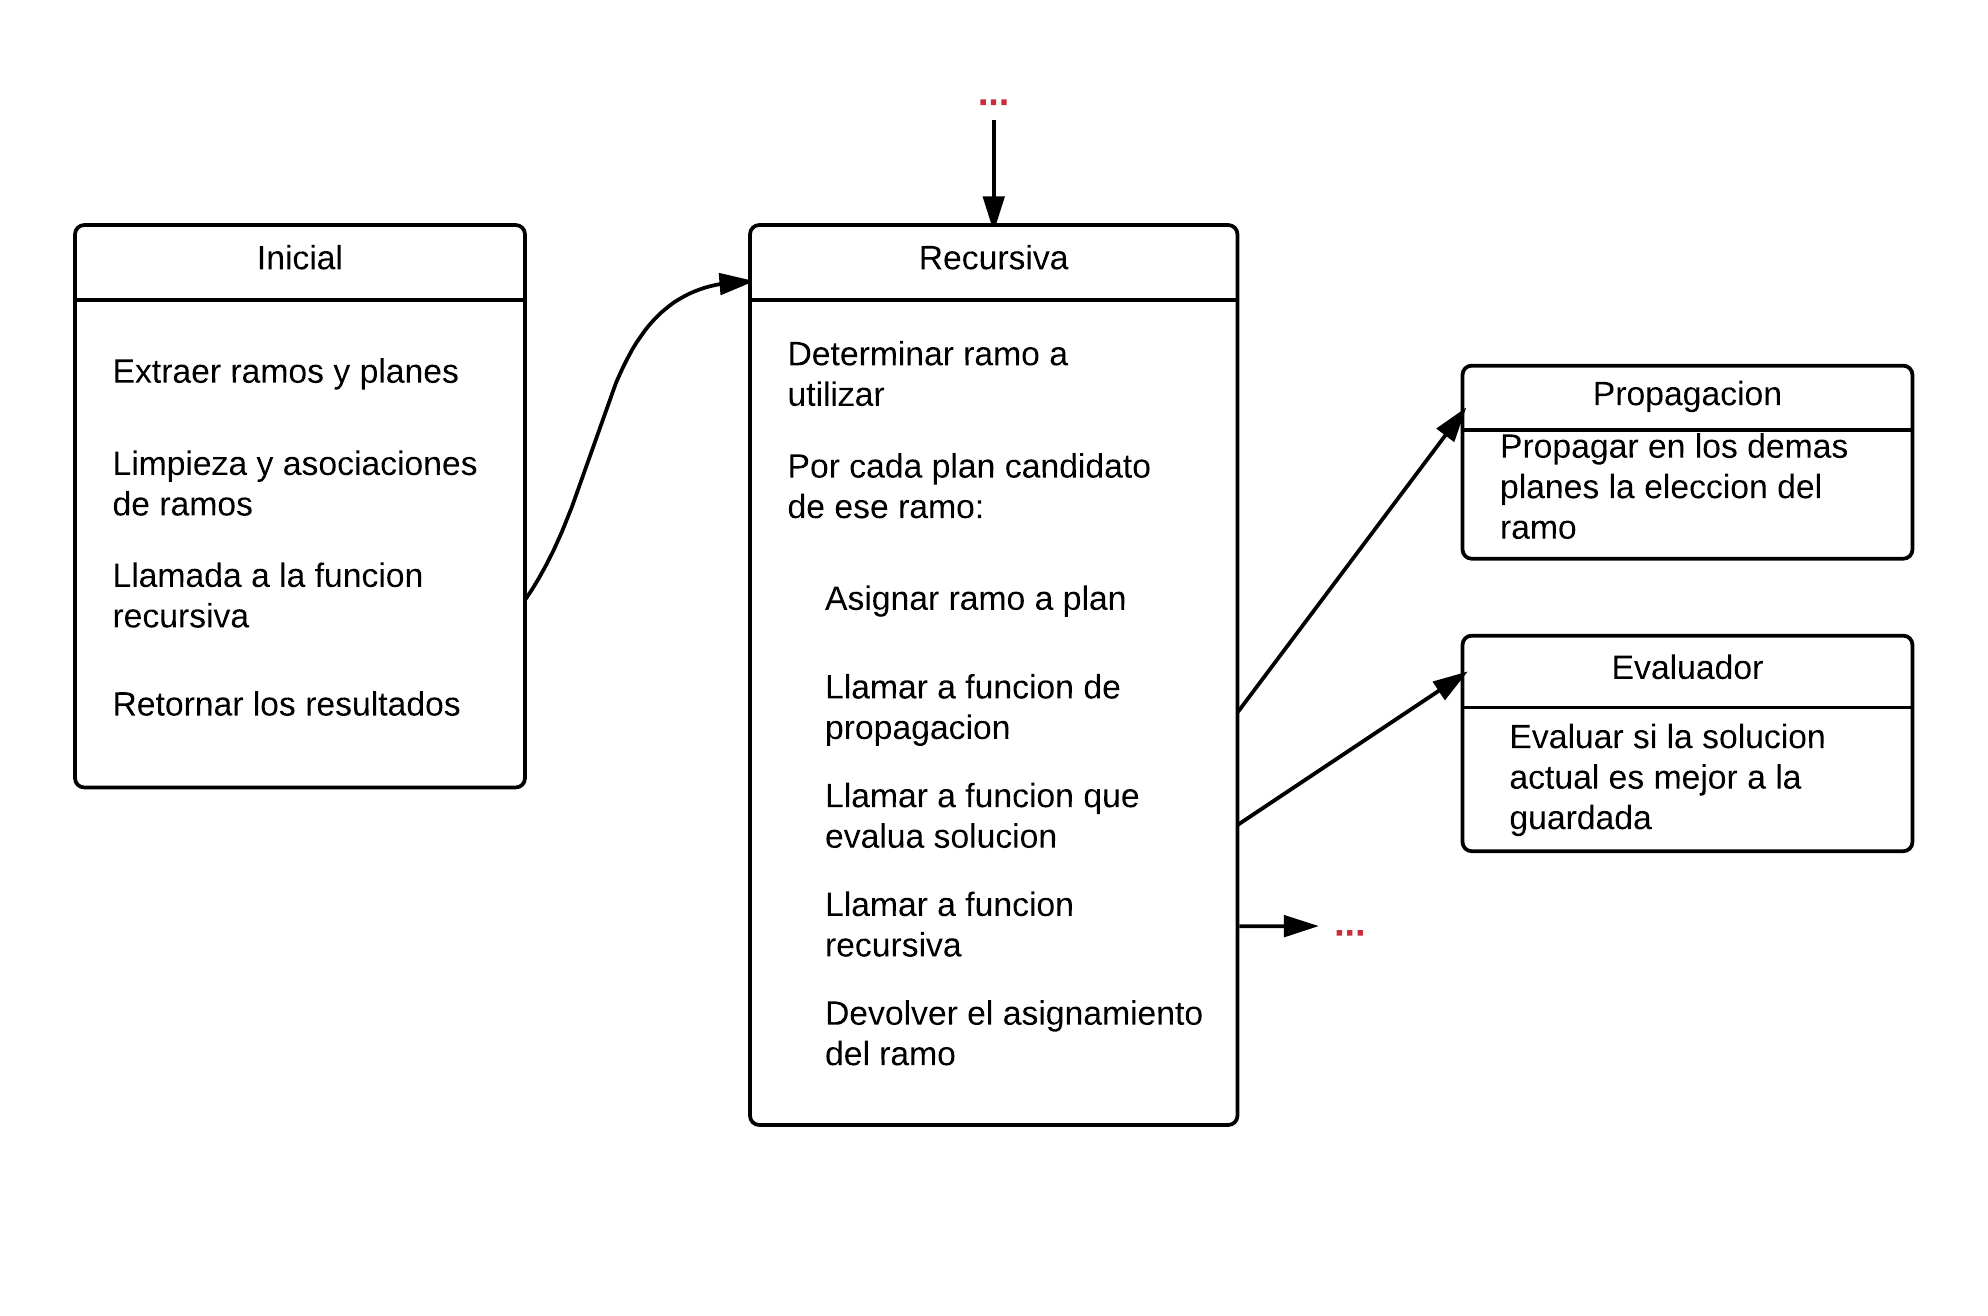
\includegraphics[scale=0.7]{imagenes/15}
	\caption{Funciones de la implementaci�n anterior y sus comportamientos.}
	\label{impl_old}
\end{figure}

En este caso, se utiliz� la misma forma de programaci�n preocup�ndose que todas las funciones tuvieran una firma similar entre ellas respetando que siempre reciban la lista de ramos y planes, y retornen la mejor soluci�n si corresponde. Adem�s, como no estaba dentro del alcance se reutiliz� la implementaci�n hecha en la funcion inicial de la implementaci�n anterior. Por lo tanto se poseen seis funciones donde tres de ellas se corresponden con las explicadas en el parrafo anterior exceptuando la recursiva debido a que se cambio el comportamiento del algoritmo.

\begin{figure}[!h]
	\centering
	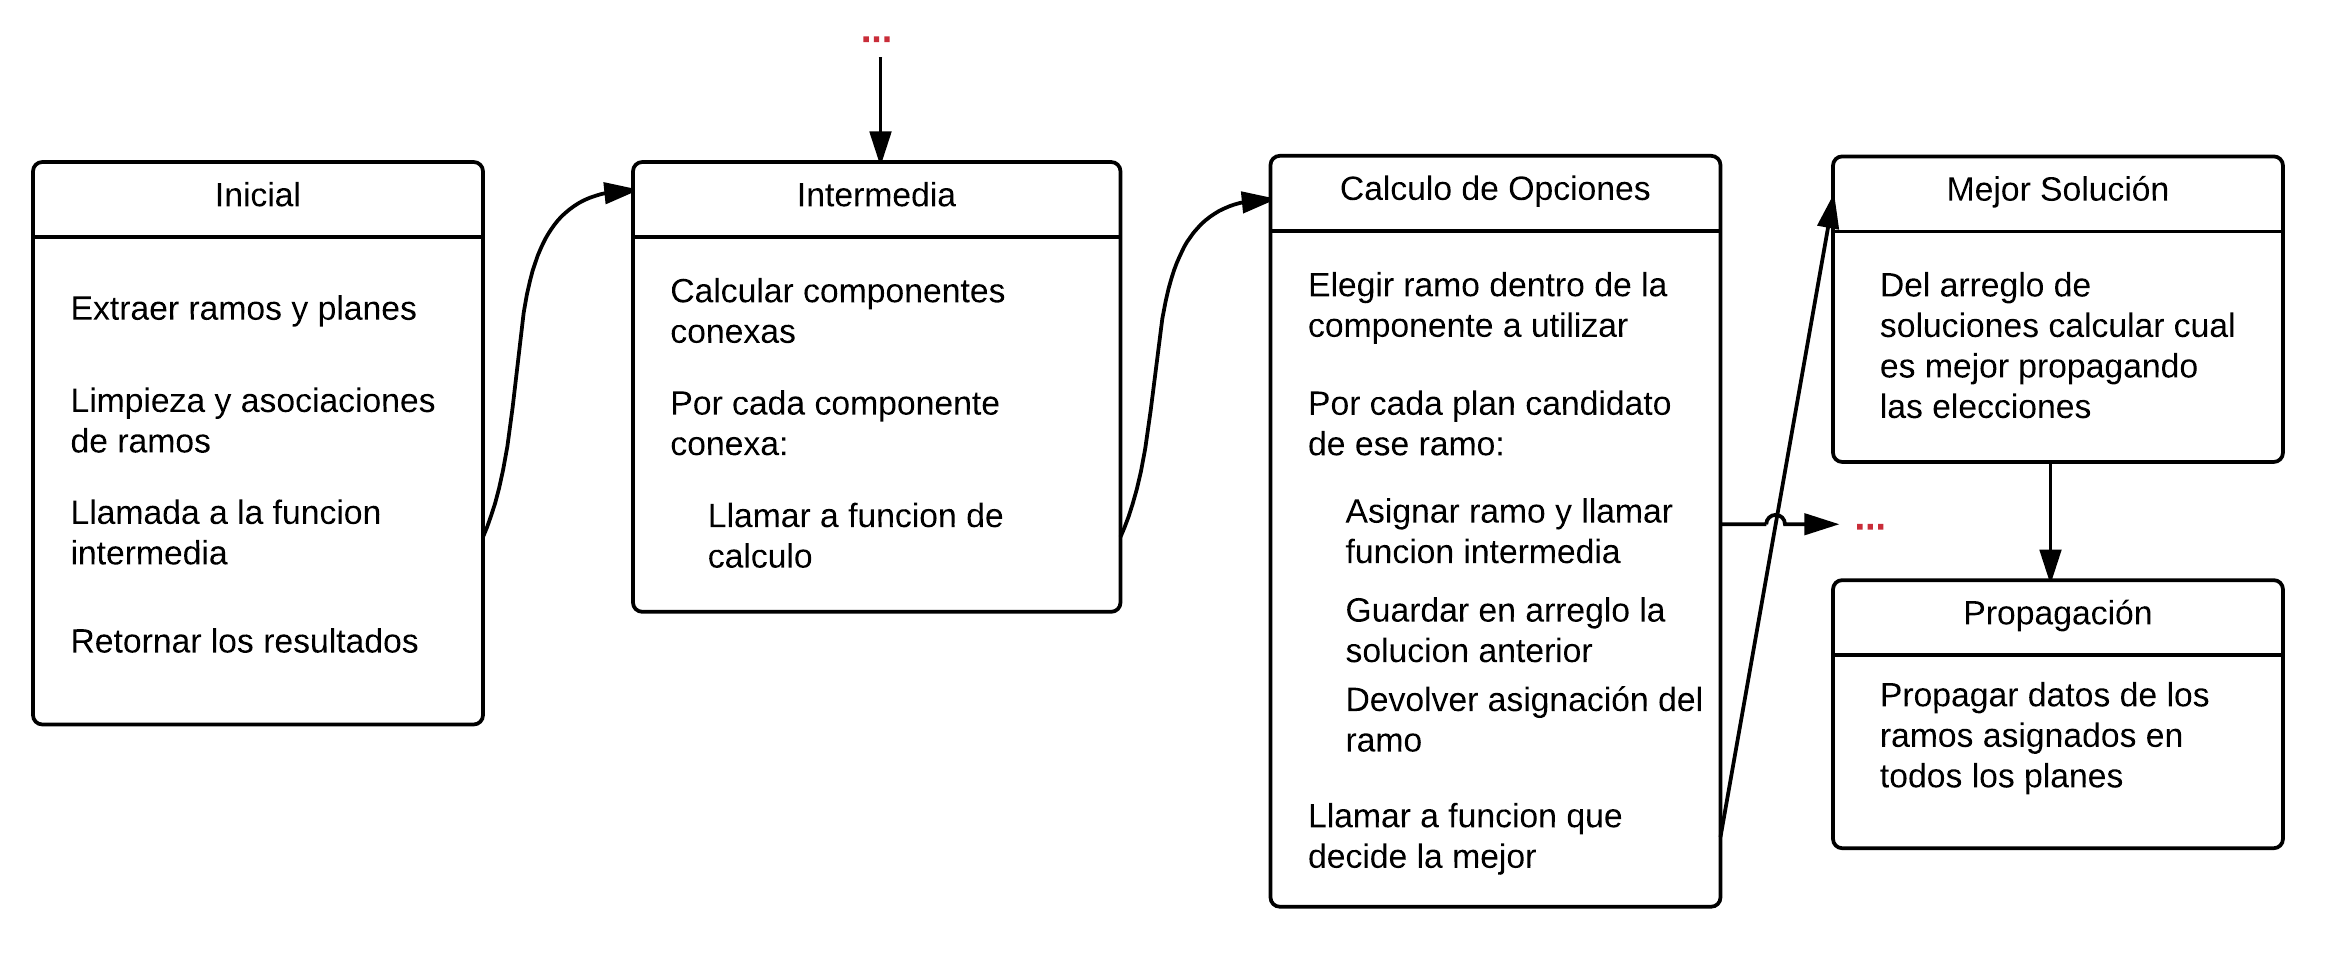
\includegraphics[scale=0.2]{imagenes/16}
	\caption{Funciones de la nueva implementaci�n y sus comportamientos.}
	\label{impl_new}
\end{figure}

Una de las funciones es el calculo de las componentes conexas donde a partir de los ramos se dividen en distintos arreglos debido a los planes que comparten. A esta funci�n siempre se le entrega la lista de todos los ramos y planes pero puede adicionarse una tercera variable opcional que dice que subconjunto de esas listas deben ser considerados para el calculo y cuales elementos deben quedan fuera.

Otra funci�n es el calculo de la mejor soluci�n a partir de un arreglo de soluciones. En ella se recibe un arreglo y en una variable auxiliar se va guardando la mejor mientras se recorre el arreglo. Al termino retorna aquella variable.

La funci�n recursiva de la implementaci�n antigua se cambio por dos funciones nuevas. La primera es el paso intermedio donde se calculan las componentes conexas y por cada una de ellas se inicia el calculo de las distintas opciones de un ramo. La segunda es la que realiza este calculo, elige un ramo y calcula todas sus opciones (llamando a la primera funci�n) generando una arreglo de posibles soluciones el cual es pasado al m�todo explicado en el p�rrafo anterior donde se calcula cual es mejor.

En la primera funci�n descrita en el parrafo anterior es donde debe ir ubicada la implementaci�n del cache. All�, se debe encontrar una firma (hash) que diferencie los elementos a guardar en memoria de manera tal de discriminar cual componente conexa generada esta repitiendo su calculo para ser extraida desde la memoria y no necesitar el llamado a la segunda funci�n.

Finalmente, se posee la funci�n que realiza un recorrido con orden posterior (post order traversal) del �rbol de planes para propagar las elecciones hechas en cada paso del segundo m�todo explicado en el p�rrafo anterior.
